\documentclass[11pt, twoside, titlepage]{book}
\usepackage[hcentering,textwidth=150mm,textheight=225mm]{geometry}
\usepackage[Bjornstrup]{fncychap}
\usepackage{graphicx}
\usepackage[colorlinks=true, 
            urlcolor=blue]{hyperref}
\usepackage{mathtools} 
\usepackage{longtable}
\usepackage{makeidx}
\makeindex 

%\usepackage[margin=1in]{geometry}
\usepackage{fixltx2e} 
\usepackage[T1]{fontenc}
\usepackage[utf8]{inputenc}
\usepackage{tikz}
\usepackage{centernot}
\usepackage{listings}
\usetikzlibrary{shadows}
\usepackage[toc,page]{appendix}
\usepackage{etoolbox}
\usepackage{wrapfig}
\usepackage{tcolorbox}
\usepackage{lipsum}
\usepackage[T1]{fontenc}
\usepackage{lmodern}
\usepackage{url}
%\usepackage[svgname]{xcolor}

\usepackage{ifpdf}
\ifpdf
\usepackage{pdfcolmk}
\fi
%% check if using xelatex rather than pdflatex
\ifxetex
\usepackage{fontspec}
\fi
\usepackage{graphicx}
%%\usepackage{hyperref}
%% drawing package
\usepackage{tikz}
%% for dingbats
\usepackage{pifont}
\providecommand{\HUGE}{\Huge}% if not using memoir
\newlength{\drop}% for my convenience
%% specify the Webomints family
\newcommand*{\wb}[2]{\fontsize{#1}{#2}\usefont{U}{webo}{xl}{n}}
%% select a (FontSite) font by its font family ID
\newcommand*{\FSfont}[1]{\fontencoding{T1}\fontfamily{#1}\selectfont}
%% if you don�t have the FontSite fonts either \renewcommand*{\FSfont}[1]{}
%% or use your own choice of family.
%% select a (TeX Font) font by its font family ID
\newcommand*{\TXfont}[1]{\fontencoding{T1}\fontfamily{#1}\selectfont}
%% Generic publisher�s logo
\newcommand*{\plogo}{\fbox{$\mathcal{PL}$}}
%% Some shades
\definecolor{Dark}{gray}{0.2}
\definecolor{MedDark}{gray}{0.4}
\definecolor{Medium}{gray}{0.6}
\definecolor{Light}{gray}{0.8}
%%%% Additional font series macros
\makeatletter
%%%% light series
%% e.g., kernel doc, section s: line 12 or thereabouts
\DeclareRobustCommand\ltseries
{\not@math@alphabet\ltseries\relax
\fontseries\ltdefault\selectfont}
%% e.g., kernel doc, section t: line 32 or thereabouts
\newcommand{\ltdefault}{l}
%% e.g., kernel doc, section v: line 19 or thereabouts
\DeclareTextFontCommand{\textlt}{\ltseries}
% heavy(bold) series
\DeclareRobustCommand\hbseries
{\not@math@alphabet\hbseries\relax
\fontseries\hbdefault\selectfont}
\newcommand{\hbdefault}{hb}
\DeclareTextFontCommand{\texthb}{\hbseries}
\makeatother

\newcommand*{\titleGM}{\begingroup% Gentle Madness
%\begin{titlepage}
\thispagestyle{empty}
\drop = 0.1\textheight
\vspace*{\baselineskip}
\vfill
\hbox{%
\hspace*{0.2\textwidth}%
\textcolor{Light}{\rule{19pt}{\textheight}}
\hspace*{0.05\textwidth}%
\parbox[b]{0.75\textwidth}{
\vbox{%
\vspace{\drop}
{\noindent\HUGE\bfseries MSCViewer V%VERSION%\\[0.5\baselineskip]
User Manual}\\[2\baselineskip]
%{\HUGE\bfseries User Manual}\\[4\baselineskip]
%{\Large }
\par
\vspace{0.5\textheight}
{\noindent Roberto Attias}\\[\baselineskip]
}% end of vbox
}% end of parbox
}% end of hbox
\vfill
\null
%\end{titlepage}
\endgroup}



\newcommand{\prog}{MSCViewer} 

\newcommand{\mscevent}{\texttt{@event}}
\newcommand{\mscentity}{\texttt{@entity}}
\newcommand{\naive}{ na\"{\i}ve}
\newcommand{\closebutton}{
\includegraphics[height=.7\baselineskip]{images/close1.png}}
\newcommand{\tblimg}[1]{\raisebox{-.5\height}{\includegraphics[height=.2in]{#1}}}

\newenvironment{Sidebar}[1][r]
  {\wrapfigure{#1}{0.5\textwidth}\tcolorbox}
  {\endtcolorbox\endwrapfigure}
  
\newcommand*\keystroke[1]{%
  \tikz[baseline=(key.base)]
    \node[%
      draw, 
      fill=white,
      drop shadow={shadow xshift=0.25ex,shadow yshift=-0.25ex,fill=black,opacity=0.75},
      rectangle,
      rounded corners=2pt,
      inner sep=1pt,
      line width=0.5pt,
      font=\scriptsize\sffamily
    ](key) {#1\strut}
  ;
}

\newcommand{\todo}[1]{\textit{#1}}
\newcommand{\defterm}[1]{\textit{#1}\index{#1}}

%\title{\prog{} v1.0} \author{ Roberto Attias  \\
%    User Manual
%    }
\date{\today}  

\definecolor{dkgreen}{rgb}{0,0.6,0}
\definecolor{gray}{rgb}{0.5,0.5,0.5}
\definecolor{mauve}{rgb}{0.58,0,0.82}
\definecolor{lightcyan}{rgb}{0.83,0.97, 1}

\lstset{frame=tb,
  language=Python,
  aboveskip=3mm,
  belowskip=3mm,
  showstringspaces=false,
  columns=flexible,
  basicstyle={\small\ttfamily},
  numbers=left,
  numberstyle=\tiny\color{gray},
  keywordstyle=\color{blue},
  commentstyle=\color{mauve},
  stringstyle=\color{dkgreen},
  backgroundcolor=\color{lightcyan},
  frame=shadowbox,
  xleftmargin=2em,
  framexleftmargin=1.5em, 
  rulesepcolor=\color{gray},
  breaklines=true,
  breakatwhitespace=true,
  tabsize=3,
  escapeinside={(*}{*)}
}

\makeatletter
\renewcommand\tableofcontents{
    \if@twocolumn
      \@restonecoltrue\onecolumn
    \else
      \@restonecolfalse
    \fi
    \chapter*{\contentsname}%
        \@mkboth{%
           \MakeUppercase\contentsname}{\MakeUppercase\contentsname}%
    \@starttoc{toc}%
    \if@restonecol\twocolumn\fi
    }
\makeatother  

\titleGM


\begin{document}
%\maketitle
\clearpage
\thispagestyle{empty}

\include{tocnotoc} 

\cleardoublepage

\setcounter{page}{1}
% Hint: \title{what ever}, \author{who care} and \date{when ever} could stand 
% before or after the \begin{document} command 
% BUT the \maketitle command MUST come AFTER the \begin{document} command! 
%\maketitle


\chapter{Introduction}

\section{\prog}
\prog{} is a tool supporting visualization and analysis of message sequence
charts. The tool loads a text file, interprets lines containing the
\mscevent{} or \mscentity{} keywords and representing events and interactions occurring on
entities, ignoring other lines. From the interpreted lines a model is
constructed in memory. In the GUI the tool can visualize the list of enties,
from which the user can select a subset to be shown in a sequence diagram chart.
through keyboard or mouse commands the user can easily navigate through events
and interactions, search, and perform a number of other actions for browsing the
diagram.

In a design phase the user can write a concise description of one or
more flows in the inpujt language,load it in the tool, and export an image to 
be used for documentation.

By instrumenting certain point in the program or application with syslogs,
printf, traces or any other mechanism avaliable, the user can generate run the
application and generate the input file for \prog{}. In this case the input
file contains flows corresponding to actual executions, which could be visually
inspected for verification.

Visual inspection of flows from execution logs is useful, but doesn't scale for
debugging, as it requires a human operator familiar with the expected flows.
When applications are large enough, their development might be distributed
across multiple teams, with only few members fully aware of cross-component
flows. To address this problem \prog{} is integrated with a Python interpreter
and supports execution of scripts which can browse the model and perform any
sort of validation. In addition, a set of classes is provided to support a
concise description of expected flows. With these mechanism the user can create
validation script to be executed in the tool on the model created from execution
logs, automatically validating their correctness. Scripts can also be executed
from command line, without any GUI visualization, supporting batch validations
and product smoke-testing.

\section{Message Sequence Charts and Flows}
A large class of products and application is composed by multiple concurrent
entities. For example a web application may be composed by a front-end running
in a browser, a backend web server and a database. The user interacts with the 
frontend, which in turn interacts with the backend. The backend interacts with
the database. We refer to elements involved in the interactions as 
\defterm{Entities}, and the sequence of interactions among entities required to
perform a functionality as \defterm{Flow}. 

\begin{figure}[ht!]
  \centering
  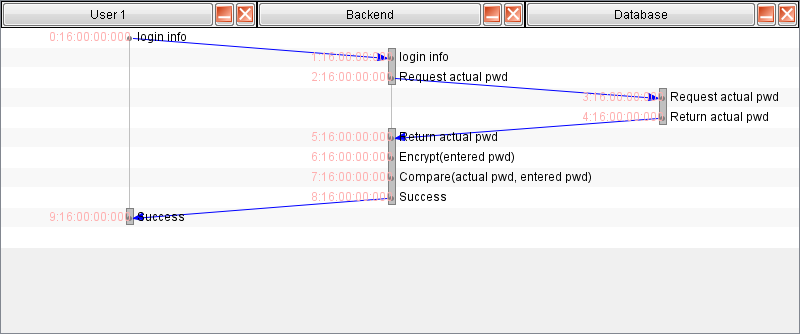
\includegraphics[width=0.5\textwidth,natwidth=1024,natheight=600]{images/simple-flow.png}
  \caption{A simple flow example}
  \label{fig:simple-flow} 
\end{figure}  
 
Fig~\ref{fig:simple-flow} shows, as an example, the flow involving a user
logging into a server which stores users information in a database. 
In complex concurrent system multiple homogeneous or heterogeneous flows
spawning tens or hundreds of entities may be in execution at any point in time.  
  
When designing, implementing and debugging such a complex system flows play a
very important role in the entire development cycle. 

In the design phase is fairly common to represent expected flows in a design
document through some variation of Message Sequence Charts
\footnote{for more information on Message Sequence Chart see~
\href{http://en.wikipedia.org/wiki/Message\_sequence\_chart}
{http://en.wikipedia.org/wiki/Message\_sequence\_chart}}, such as the one shown
in fig~\ref{fig:simple-flow}.

In the implementation phase the developer can sprinkle calls to a
tracing/logging \footnote{ for more information about tracing vs.
logging
see~\href{http://en.wikipedia.org/wiki/Tracing\_(software)}
{http://en.wikipedia.org/wiki/Tracing\_(software)}} infrastructure
around the main points of flows.
  
At debug time
the user can then browse the various log files and mentally reconstruct and
verify flows. If not properly supported by a tool this exercise can be complex
and time-consuming, as the user has to reassemble flows identifying relevant
information often diluted in hundreds of lines of unrelated logs. To add to this
complexity, flows may not always be purely sequential like the one shown in
fig~\ref{fig:simple-flow}. 

For example, fig~\ref{fig:concurrent-flow} shows a user requesting the
instantiation of a virtual machine to an hypotetical VM Manager. the VM Manager
requests asynchrously resources (disk space, CPU, memory) to a Resource Manager
and an image for the VM to a VM Repository. When the resources and VM image are
provided, VM Manager spawns the VM.

\begin{figure}[ht!]
  \centering
  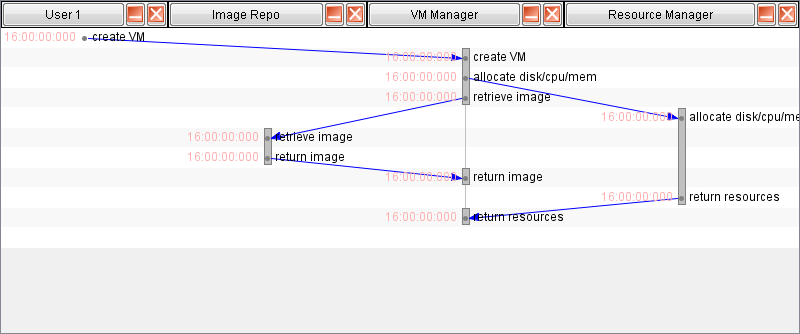
\includegraphics[width=0.5\textwidth,natwidth=1024,natheight=600]{images/concurrent-flow.png}
  \caption{A flow with two concurrent branches}
  \label{fig:concurrent-flow} 
\end{figure}  

Note that the flow could also happen in different ways. For example, 
the response from the Image Repo could reach VM Manager before the response from
the Resource Manager. The implication of this consideration is that verifying
whether a flow happened as expected doesn't always amount to simply checking
whether certain string appear in a specific total order in the logs. Sometimes
events (i.e. log lines) have only a partial order, or some parts may be
optional, for example in case of an \textit{if} vs. \textit{else} branch taken 
in the code.

Capturing flows at design time is very
important to properly document how a system composed by multiple concurrent
elements operate. Validating flows in logs of runtime executions is crucial to
guarantee a complex system is operating as expected. \prog{} was designed  to
support this.

%\section{Tracing and Logging}
%\prog{} Accepts in input is either hand written to capture a desired flow at design time,
%case the program has produced information through some infrastructure
%or generated by running code, to capture an actual execution. In the latter
%The definition of tracing and logging are not always  

\section{History and Acknowledgements}
Work on \prog{} was started around 2010 at CISCO. The idea was to develop a tool
for usage during development of the control plane for the NCS-6000, CISCO 
last-generation core router, specifically to address the problem of
automatically identifying potential problems in flows and reducing the triaging 
time and amount of resources required. While the tool was started as a personal
initiative, it has found good adoption by some communities in the company. 

Before 2010, I had worked on other tools with some common aspects, so \prog{} can
be considered the result of an effort started around 2001 
(no code or IP from those early efforts has been used in \prog{}). 

As of Sept. 2014 CISCO has gracefully consented to release \prog{} in the
open-source. 

I want to thank the following people for their ideas, suggestions, feedback and
support during development of \prog{}:

\begin{itemize}
\item Akash Deshpande and Marco Zandonadi, whose collaboration in CISCO and before
has helped shaping \prog{} to its current form;

\item Edward Conger, for his suggestions, observation and his ability to push
the boundary of \prog{} and other tools I developed;

\item the CISCO managment, in particular Sunil Khaunte, Feisal Daruwalla, Satish
Gannu, Sohyong Chong and Robert Krohn, for their support during the developement
of \prog{} and for facilitating its release as open source.
\end{itemize} 

\chapter{Getting Started} 
In this chapter we will start familiarizing with \prog{} concepts through some
examples. The files used in the examples are located in the \texttt{examples/}
directory of the distribution.

\section{Your First Sequence Diagram}
The following is a simple input file for \prog{}:
\lstinputlisting{../../examples/lst1.msc}
Each line defines an \defterm{event}, i.e. an occurrence of something relevant
in an entity. The syntax consists in the \mscevent{} token followed by a JSON
object (see \href{http://json.org/}{http://json.org/} for more information about the JSON format).

Line 1 defines a \defterm{local} event, which is not part of any interaction
with other entities. The value of the \mscentity{} key indicates the entity
this event belongs to. There is no explicit sytax to define an entity: as it
parses events, \prog{} creates entities the events belong to.

Line 2 defines an event which is part of an interaction. More specifically, this
event is the \defterm{source} (or \defterm{cause}) for the interaction, as
indicated by the presence of the \texttt{src} key. Line 3 defines a
\defterm{destination}, or \defterm{effect}, as indicated by the presence of the
\texttt{dst} key. An interaction is an ordered pair composed by a cause and an
effect event. 

\section{Running \prog}

We can now start \prog{} with this input file. Assuming the current directory is
the top directory of the  distribution, run:

\begin{lstlisting}
bin/(*\MakeLowercase{\prog}*) examples/lst1.msc
\end{lstlisting}

\begin{figure}[ht!]
  \centering
  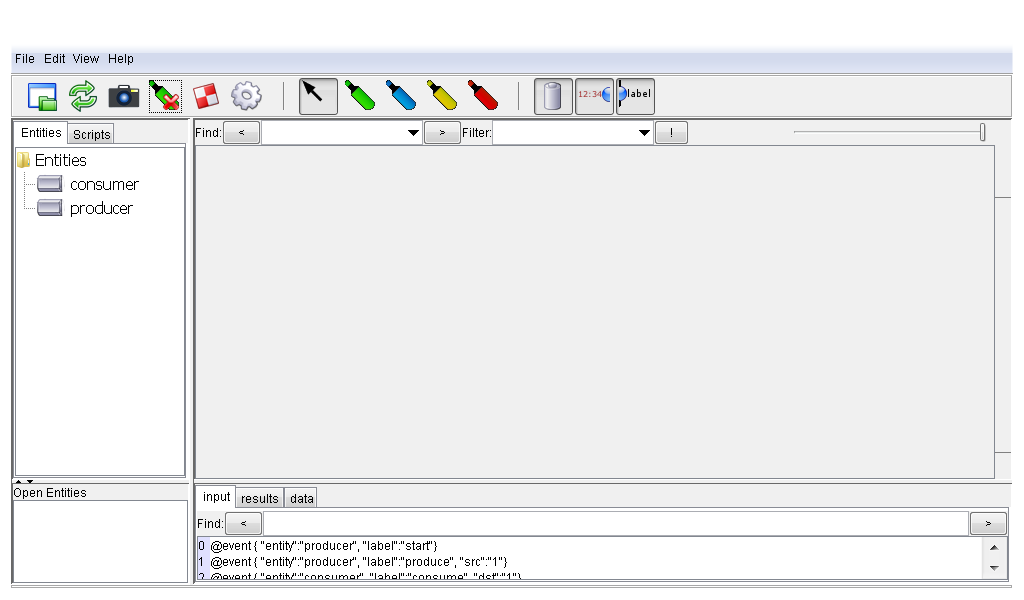
\includegraphics[width=0.5\textwidth,natwidth=1024,natheight=600]{images/gui-ex1.png}
  \caption{\prog{} GUI with \texttt{lst1.msc} loaded.}
  \label{fig:gui-lst1}
\end{figure}

Fig.~\ref{fig:gui-lst1} shows the GUI in its initial state.  The bottom-right
area shows the content of the input file, while the top-left tree shows the various
entities. Double-click on the \texttt{producer} and \texttt{consumer} entities
to open them in the diagram area, in the top-right part of the window
(fig.~\ref{fig:gui-lst1-open}). Each entity is shown in a column, with events
interleaving each other across entities. Columns can be sorted by dragging them
from their header (the part showing the entity name), and closed by clicking on
the   \closebutton{} button. Clicking on an event selects it; the selection can
be moved to the previous/next event for an entity by pressing respectively the
\keystroke{SHIFT} \keystroke{$\uparrow$} and \keystroke{SHIFT}
\keystroke{$\downarrow$} key combinations. To navigate from a source or
destination event to the paired event in an interaction use the 
\keystroke{SHIFT} \keystroke{$\leftarrow$} or \keystroke{SHIFT} \keystroke{$\rightarrow$}.

\begin{figure}[ht!]
  \centering
  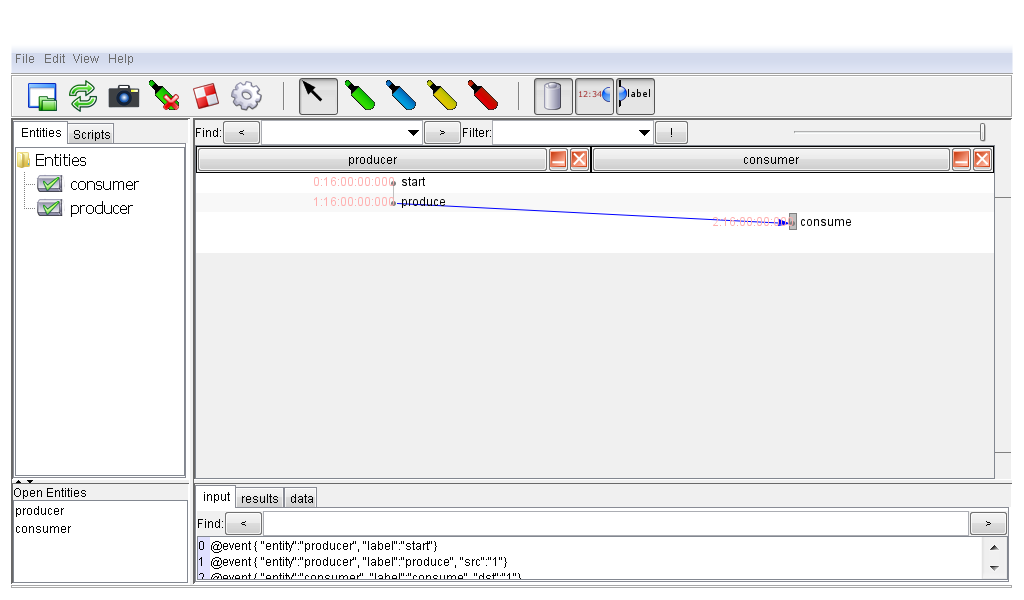
\includegraphics[width=0.5\textwidth,natwidth=1024,natheight=600]{images/gui-ex2-open.png}
  \caption{The user has opened all the entities in the diagram}
  \label{fig:gui-lst1-open}
\end{figure}


Try closing the \texttt{consumer} entity by clicking on the \closebutton{}
button. As the destination entity is now closed, the interaction outgoing from
the producer is shown as an arrow stub. In this case, it is pretty obvious who the
destination entity is, but in more complex scenarios there can be hundreds of
entities, and it wouldn't be easy to know which one to open from the entities tree. In
this situation the keyboard navigation cames handy. Select the interaction stub,
then press \keystroke{SHIFT} \keystroke{$\rightarrow$}: ``pushing'' on the
tip/base of an interaction stub for which the destination/source entity is not
open causes the entity to be opened.

\section{Topological Sorting}
In the diagram in fig.~\ref{fig:gui-lst1-open} events appear in the 
same order in which they were in the file. However, this is not always
the case. Select the \texttt{File/Open...} menu item, and from the file
selection widget open the \texttt{lst2.msc} file. As shown in the input area,
this file is the same as \texttt{lst1.msc}, except that the last two lines have
been swapped. Despite the fact that the destination for the interaction is
listed before the source, opening the two entities will show the same diagram as
before: \prog{} tries to preserve cause-effect ordering among events by applying
a topological sort to the events as they're loaded. It is possible to write
input files with create circular dependencies of events, resulting in the
impossibility of performing a topological sorting. In this case \prog{} reports
an error upon loading the file and skips the sorting. This case is captured in
\texttt{lst3.msc}, shown in fig.~\ref{fig:gui-lst3}

\begin{figure}[ht!]
  \centering
  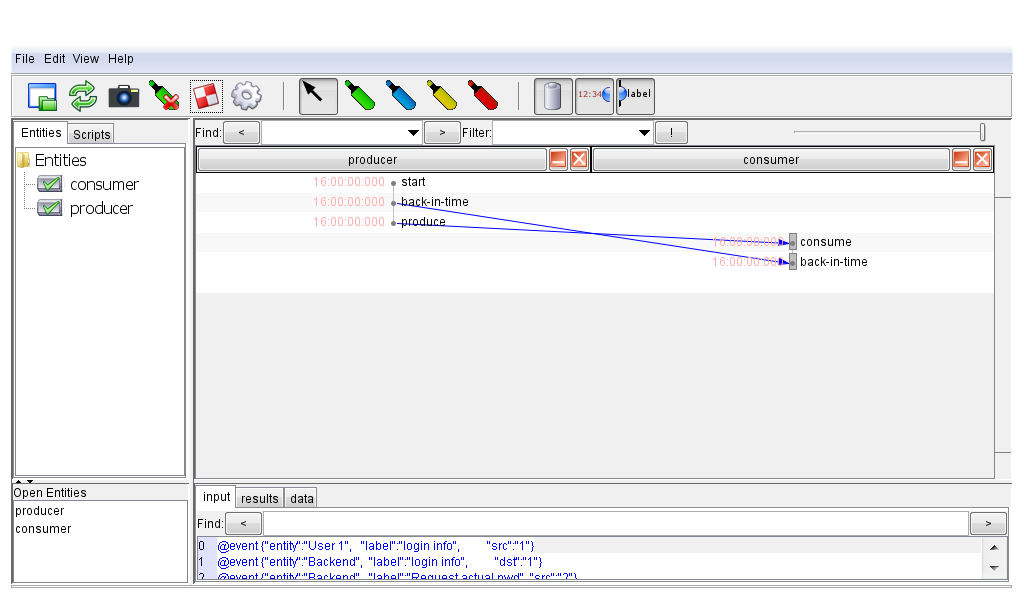
\includegraphics[width=0.5\textwidth,natwidth=1024,natheight=600]{images/gui-ex3-cycle.png}
  \caption{Diagram with circular dependencies caused by interactions}
  \label{fig:gui-lst3}
\end{figure}

\section{Timestamps}
It is possible to associate timestamps to each event throught the \texttt{time}
key. The value can assume different formats, as shown in \texttt{lst4.msc},
visible in fig.~\ref{fig:gui-lst4}. \prog{} internally converts the units
indicated in the input files into nanoseconds. By default timestamps are shown
to the left of events in a \texttt{hh:mm:ss} format. The format can be changed
through the \texttt{view/Preferences...} menu item.

%\lstinputlisting[language=Java]{../../examples/lst4.msc}
\begin{figure}[ht!]
  \centering
  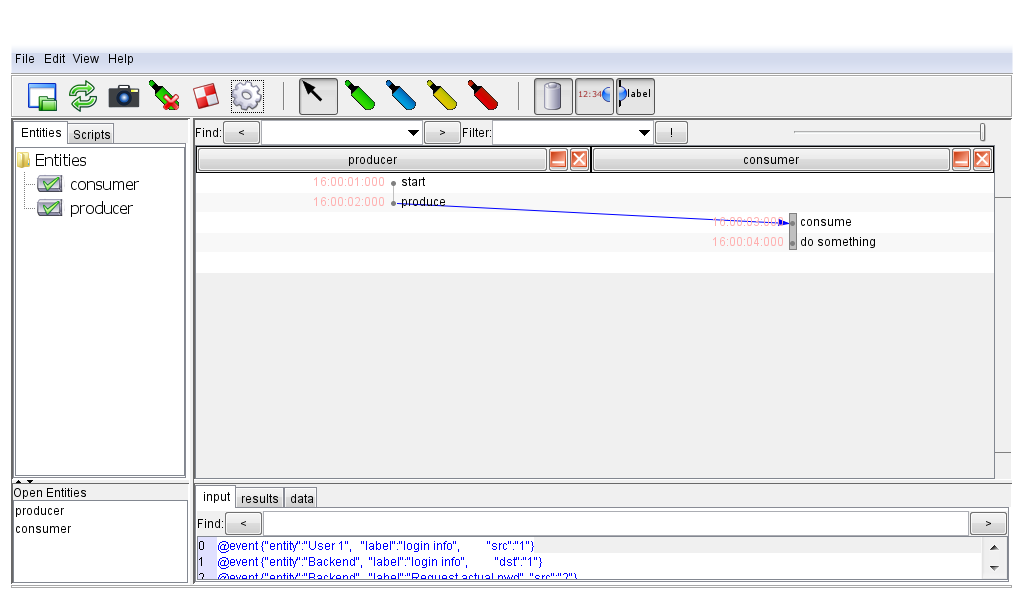
\includegraphics[width=0.5\textwidth,natwidth=1024,natheight=600]{images/gui-ex4-time.png}
  \caption{Diagram with timestamps associated to events.}
  \label{fig:gui-lst4}
\end{figure} 


\section{Associating Data to Events}
To associate some data to an event, use the \texttt{data} key. The value is a
JSON object that will be visualized in the bottom-right area, in the
\texttt{Data} tab. For example, loading the following input file  and selecting
the third event results in the screen as shown in fig.~\ref{fig:gui-lst5}:

\begin{minipage}{\linewidth} 
\lstinputlisting{../../examples/lst5.msc}
\end{minipage}


\begin{figure}[ht!]
  \centering
  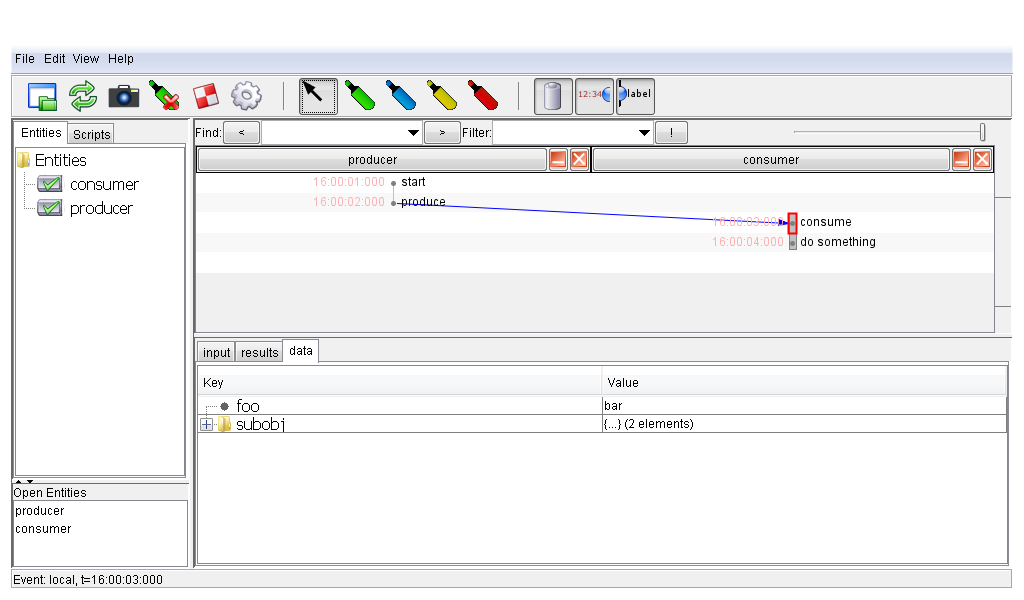
\includegraphics[width=0.5\textwidth,natwidth=1024,natheight=600]{images/gui-ex5-data.png}
  \caption{The Data view showing data associated to the selected event}
  \label{fig:gui-lst5}
\end{figure}

\section{Orphaned Interactions}
When collecting traces from a system it is possible that either the even
representing a cause or the one representing an effect for an interaction goes
missing. This can be caused by multiple reasons, such as the fact that a trace
has wrapped around (typically traces don't grow indefinitely, but rather wrap
around, loosing older information), or that traces for one of the two entity
involved in the interaction are not available. We will refer to interactions for
which only one of the two events is available as \defterm{Orphaned
Interactions}.
\prog{} visualizes orphaned interactions as dashed arrow stubs outgoing or
incoming into the only available event.


\chapter{\prog{} Model}
This chapter provides a more formal definition of the \prog{} model. 

\section {Entity}
An \defterm{entity} is an autonomous execution entity such as a thread or state
machine. In MSCViewer entities can be defined hierarchically. For example, in a
router a node entity might contain a process entity, containing  a thread
entity, containing a state machine entity. An entity is characterized by a name,
a unique ID and a set of events. The ID of an entity is composed by the ID of
the parent, a slash (\texttt{/}) and an identifier. In other words, entity IDs
have a namespace similar to a filesystem path.
Let's consider the example shown in table~\ref{tab:entities}:
 
\begin{center}
    \begin{table}[h]
    \centering
    \label{tab:entities}
    \begin{tabular}{ | l | l | l | l |}
    \hline
    ID & Name\\ 
    \hline
    0       & Node0 \\  
    1       & Node1 \\  
    0/1234  & Node0/DS \\
    0/1236  & Node0/DS \\
    1/1234  & Node1/DS \\
    \hline
    \end{tabular}
    \caption{Example of entities}
    \end{table}
\end{center}

Here we have two nodes, named \texttt{Node0} and \texttt{Node1}. The entity IDs
are respectively 0 and 1, while their names are \texttt{Node0} and
\texttt{Node1}. 

On the first node two processes are running, the first with PID
1234, the second with PID 1236. The IDs for the corresponding entities are
\texttt{0/1234} and \texttt{0/1236}. The processes are instances of the same
executable called DS, so the entity names are \texttt{Node0/DS} and
\texttt{Node0/DS}. 

On the second node a single instance of \texttt{DS} is running, with ID
\texttt{1/1234} and name \texttt{Node1/DS}

It's worth mentioning that \prog{} does not have any semantic knowledge of
concept such as nodes, processes, or threads, and the model could be used to
represent any kind of problem domain. \prog{} understands only the concept of
hyerarchical IDS and names where elements in the hyerarchy are separated by
slashes.

Some entities can have an extra attribute characterizing them as clock sources.
This indicates that the entity and all its descendants are on
the same clock domain, hence sharing the same clock. As an example, a group of
computational nodes may have a shared system clock (via software or dedicated
hardware), in which case a system root entity could be used to represent this.
In other scenarios a set of nodes may have a loose clock synchronization (for
example via NTP), in which case entities representing nodes could be clock
sources for children representing processes running on the node.


\section {Event} 
An event is an occurrence of some relevance happening to an entity. Examples of
event are the state transitions in state machines or receiving or sending a
message. An event is always characterized by a timestamp, a label, and a type.
The timestamp is relative to the clock source the entity belongs to. The label is a
human-readable message providing information about the event. They type is an
identifier representing formally the specific type of the event, used for
example to select how to visually render the event in the sequence diagram 
(see~\ref{sec:rendering}). In addition to these mandatory attributes, an event
may have a dictionary of extra attributes. Rendering code or model browsing code can retrieve these
attribute to perform special tasks.

\subsection{Events Partial Order}
\label{events-partial-order}
Theoretically all events within an clock domain are fully ordered in a
``happened-before'' relationship by their timestamp. In reality however high
event granularity, low clock resolution, or the presence of multiprocessing capabilities can result in
multiple events with the same timestamp. For example a trace may
have been generated for a computational node where have two processes have an
event happening exactly at the same timestamp. This means that model events are
a \href{http://en.wikipedia.org/wiki/Partially_ordered_set}{Partially Ordered
Set} where $ev_i < ev_j$ if at least one of the following conditions is true:

\begin{itemize}
  \item $ev_i$ and $ev_j$ belong to the same clock domain and $t(ev_i) <
   t(ev_j)$
   \item  $\exists$ an interaction $I$ such that $(ev_i \rightarrow ev_j)$ 
   \item $\exists ev_1\ldots ev_n$ such that $ev_1=ev_i,\quad ev_n=ev_j,\quad
   ev_k<ev_{k+1} \quad \forall k \in (1 \ldots n-1)$
\end{itemize}

Upon parsing the model from the input file MSCViewer applies the Kahn 
\href{http://en.wikipedia.org/wiki/Topological_sorting}{topological sorting
algorithm} according to the partial order specified above. In the algorithm
however the set $S$ set is replaced with a FIFO where elements are added in the
order in which they are defined in the input file. This, and the assumption that
the input file was sorted on timestamps, guarantees that events with the same
timestamp and no incoming edges in the graph will not be shuffled around. 

The sorted events output by the algorithm are stored in an array which reflects
the visualization order.

The topological sorting is particularly useful when the input data is produced
by entities with different clock sources. For example, an input file may be
produced by joining traces collected on two separate Linux nodes. Even when
nodes are synchronized through NTP, there may be a small drift resulting in the
tracing of a source event having a timestamp larger than the corresponding to
the tracing of the destination event. A simple merging of the two traces based
on timestamp would produce a model where cause and effect are in the opposite
order (with the arrow representing the interaction going from bottom to top).
The topological sorting takes care of this problem. Note that the timestamps
associated to the events are not modified, hence while the arrow flows from top
to bottom, the source will still show up with a timestamp greater than the
destination. Computing the actual offset between the two nodes is not trivial
if not impossible, and anyway correcting the timestamp may confuse the user. 

\section {Interaction}

An interaction is a tuple $(ev_i, ev_j, type)$ where:
\begin{itemize}
  \item $ev_i$ is called the {\it source} or {\it cause} event, and the entity
  the event belongs to is called the {\it source entity};
  \item $ev_j$ is called the {\it destination} or {\it effect} event, and the
  entity the event belongs to is called the {\it destination entity}
  \item $type$ is an identifier characterizing the nature of the interaction
  (for example \texttt{message}, or \texttt{creation})
\end{itemize}
In the model adopted interaction implies a causality between the source and
destination event, hence $(ev_i, ev_j, T) \centernot\implies (ev_j, ev_i, T)$. 

Note also that the model allows source and destination event to belong to the
same entity.

An example of interaction type is a message-passing. In this case the source
event captures the sending of the message, while the destination event captures
the reception. Another example is a state machine instantiation:
in this case the creating entity would have an ``sm instantiation'' event, while
the created state machine would have a first event corresponding to its birth.
In this case, clearly, the state machine entity would be a children of the
creator entity. An example where source and destination events belong to the
same entity is initiation and completion of a DMA operation. 
Note that the model allows for additional events
to be present between the source and destination event for an interaction.

In the model interactions are captured with an interaction ID attribute
associated to the source and destination events. This attribute has the same
value (a unique id) for events belonging to the same  interaction.

The model allows for an event to be the source of multiple interactions, but
the destination to only one interaction. events with multiple outgoing
interaction can be used, for example, to capture multicast messaging.

In this document we will in some cases use the notation $(A_{e_1} \rightarrow
B_{e_2})$ to represent an interaction between an event $e_1$ on entity $A$ and
an event $e_2$ on entity $B$

\section{Input Language}
\prog{} can load a single file containing description of events for multiple
entities and build a model in memory. The input file is composed by lines of
text. \prog{} ignores any line not containing the \mscevent{} or
\mscentity{} word. This allows to load trace files which might contain
a mix of trace lines catered to \prog{} and unrelated trace lines.

An event is described in the input language by a line containing the
\mscevent{} followed by a JSON object. If the reader is not familiar
with this format, it is explained here: \href{http://json.org/}{http://json.org/}
   
\prog interprets certain keys-value pairs in the JSON objects in order to build
the entity/event/interaction model. 

For events, the following keys are interpreted:
 

\begin{center}
    \begin{longtable}{ll}
    \hline
    \textbf{Key:}         & \texttt{entity} \\
    \textbf{Type:}        & String \\
    \textbf{Mandatory:}   & y\\
    \textbf{Example:}     & \texttt{"id":"node0/producer\_1"}\\
    \textbf{Description:} &
    \begin{minipage}[t]{0.8\columnwidth}%
        an identifier for the entity this event belongs to. identifiers can contain slash to indicate hierarchy of entities.\\
    \end{minipage}    
    \tabularnewline
    \hline
    \textbf{Key:}         & \texttt{label} \\
    \textbf{Type:}        & String \\
    \textbf{Mandatory:}   & y\\
    \textbf{Example:}     & \texttt{label":"operation competed"}\\
    \textbf{Description:} &
    \begin{minipage}[t]{0.8\columnwidth}%
        a label specifying some immediate info about this event. In MSCViewer the label is shown on the right 
        of the icon representing the event.\\
    \end{minipage}    
    \tabularnewline
    \hline
    \textbf{Key:}         & \texttt{time} \\
    \textbf{Type:}        & String \\
    \textbf{Mandatory:}   & n\\
    \textbf{Example:}     & \texttt{"time":"1542532s"}\\
    \textbf{Description:} &
    \begin{minipage}[t]{0.8\columnwidth}%
        a timestamp for the event.  It's an integer number followed by a unit qualifier: "s" (seconds), "ms" 
        (milliseconds), "us" (microseconds) or "ns" (nanoseconds). The timestamp is interpreted as elapsed time 
        since the Unix Epoch . If the timestamp is not present inside the JSON object, it is expected to be 
        present before it in one of the formats supported by syslog.  time is shown in MSCViewer at the right 
        of the event icon. \\
    \end{minipage}    
    \tabularnewline
    \hline
    \textbf{Key:}         & \texttt{type} \\
    \textbf{Type:}        & String \\
    \textbf{Mandatory:}   & n\\
    \textbf{Example:}     & \texttt{"type":"Timer"}\\
    \textbf{Description:} &
    \begin{minipage}[t]{0.8\columnwidth}%
        If present, the value specifies a distinct type for the event. Events of different types can be rendered
         by different icons in MSCViewer. Icons can be provided by a user in a directory in the form of PNG images
          whose name matches the type name. This allows to plug domain-specific representation for events.\\
    \end{minipage}    
    \tabularnewline
    \hline
    \textbf{Key:}         & \texttt{data} \\
    \textbf{Type:}        & JSON Value\\
    \textbf{Mandatory:}   & n\\
    \textbf{Example:}     & \texttt{"data":\{"v1":10, "v2":20\}} \\
    \textbf{Description:} &
    \begin{minipage}[t]{0.8\columnwidth}%
	    Specifies some data associated to the event. For example, if the event corresponds to the sending of 
	    a message, the value here could be a JSON representation of the message. in MSCViewer data is shown in 
	    a table in the data section when the event is selected.\\
    \end{minipage}    
   \tabularnewline
    \hline
    \textbf{Key:}         & \texttt{src} \\
    \textbf{Type:}        & JSON Value\\
    \textbf{Mandatory:}   & n\\
    \textbf{Example:}     & 
        \begin{minipage}[t]{0.8\columnwidth}%
            \texttt{"src":"producer\_1/123"},\\
            \texttt{"src":"\{"id":"producer\_1/123", "color":"00FF00"\}} 
        \end{minipage}  \\  
    \textbf{Description:} &
    \begin{minipage}[t]{0.8\columnwidth}%
        Interactions are pairs of events. In a pair, one event contains the src key, while the other contains the 
        dst key, both with the same value. Interactions are visualized in MSCViewer as arrows going from the source
        to the destination event. The file format doesn't mandate a particular format for the value, but the value
        should be unique for an interaction (more on this in the interaction section of this document. In the 
        simplest case the value can be a string (which is a valid JSON value). When certain aspects of the 
        rendering need to be controlled, the value can be a JSON object with an "id" key identifying the unique
         interaction, and other keys (such as "color") identifying rendering aspects.\\
     \end{minipage}   
   \tabularnewline
    \hline
    \textbf{Key:}         & \texttt{dst} \\
    \textbf{Type:}        & JSON Value\\
    \textbf{Mandatory:}   & n\\
    \textbf{Example:}     & 
        \begin{minipage}[t]{0.8\columnwidth}%
            \texttt{"dst":"producer\_1/123"},\\
            \texttt{"dst":"\{"id":"producer\_1/123", "color":"00FF00"\}} 
        \end{minipage}  \\  
    \textbf{Description:} &
    \begin{minipage}[t]{0.8\columnwidth}%
        Interactions are pairs of events. In a pair, one event contains the src key, while the other contains 
        the dst key, both with the same value. Interactions are visualized in MSCViewer as arrows going from
        the source to the destination event. The file format doesn't mandate a particular format for the value,
        but the value should be unique for an interaction (more on this in the interaction section of this 
        document. In the simplest case the value can be a string (which is a valid JSON value). When certain
        aspects of the rendering need to be controlled, the value can be a JSON object with an "id" key 
        identifying the unique interaction, and other keys (such as "color") identifying rendering aspects.\\
     \end{minipage}    
   \tabularnewline
  \hline
  \end{longtable}
\end{center}
 
 
The following table shows the keys interpreted by MSCViewer for entities:

\begin{center}
    \begin{longtable}{ll}
    \hline
    \textbf{Key:}         & \texttt{id} \\
    \textbf{Type:}        & String \\
    \textbf{Mandatory:}   & y\\
    \textbf{Example:}     & \texttt{"id":"/node0/1984"}\\
    \textbf{Description:} &
    \begin{minipage}[t]{0.8\columnwidth}%
		The unique identifier for the entity \\
    \end{minipage}    
    \tabularnewline
    \hline
    \textbf{Key:}         & \texttt{name} \\
    \textbf{Type:}        & String \\
    \textbf{Mandatory:}   & y\\
    \textbf{Example:}     & \texttt{"id":"/node0/producer\_1"}\\
    \textbf{Description:} &
    \begin{minipage}[t]{0.8\columnwidth}%
        A name for the entity. Names don't need to be unique and provide a more human-readable representation for the entity\\    
    \end{minipage}    
    \tabularnewline
	\end{longtable}
\end{center}
 
   
\chapter{\prog{}  GUI}
This chapter provides a description of all the GUI elements in \prog.

\section{The Entities Tree}

\begin{figure}[ht!]
  \centering
  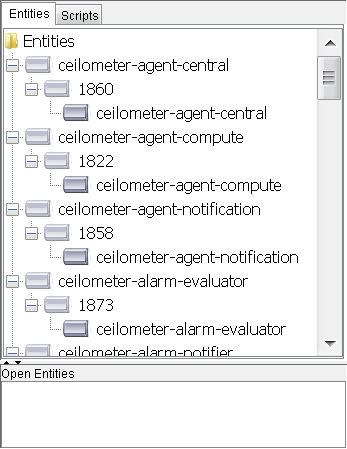
\includegraphics[width=0.3\textwidth]{images/left-pane.png}
  \caption{The Entities tree}
  \label{fig:entity-tree} 
\end{figure}  

The Entities Tree is visible on the top-left are of the GUI once an input file is loaded and the \textit{Entities} tab 
is selected. This tree shows all entities defined in the input file. An entity is defined if a \mscentity{} line is 
present or if the entity is specified in the \texttt{entity} entry of a \mscevent line. Elements of an entity 
ID separated by slashes constitute nodes in the tree. Internal nodes of the tree may have event of their own, if 
they appear as the terminal element in the \texttt{entity} entry of at least one event, or not, in which case they
just represent some relationship among the child nodes. In the latter case the node is visualized in a lighter 
shade.

For example, a system may be composed by multiple processes running in different hosts. The user may decide to 
have a log file for each process, and use a \texttt{host-id/process-id} notation for entity events. In this case,
Intermediate tree nodes for host-id will be created, but clearly there will be no events associated to them.

Double-clicking on a node corresponding to an entity with at least one event opens the entity in the Sequence 
Diagram. Double-clicking on a node corresponding to an entity already opened in the Sequence Diagram causes
it to be removed from the diagram. The following legend shows the various representations of the tree nodes:

\begin{center}
    \begin{longtable}{ll}
  	\tblimg{../../src/com/cisco/mscviewer/resources/icons/32x32/entity.png}
	& entity with at least one event, currently closed in sequence diagram\\
  	\tblimg{../../src/com/cisco/mscviewer/resources/icons/32x32/entity_open.png}
	& entity with at least one event, currently open in sequence diagram\\
  	\tblimg{../../src/com/cisco/mscviewer/resources/icons/32x32/entity_faded.png}
	& entity with no event, can't be opened in sequence diagram\\
	\end{longtable}
\end{center}


\section{The Sequence Diagram area}
The sequence diagram area is situated on the top-right part of the GUI. Entities can be opened in this area by
double-clicking on them in the Entity Tree. Open entities can be rearranged by dragging them from their 
header.

\section{The Tool Bar}
The toolbar contains the following buttons:

\begin{center}
    \begin{longtable}{ll}
	 \multicolumn{2}{l}{\textbf{Actions}} \\
	\hline
  	\tblimg{../../src/com/cisco/mscviewer/resources/icons/32x32/load.png}
	& \begin{minipage}[t]{0.8\columnwidth}
		Loads a new input file. Pressing this button causes a file chooser to open. Selecting a file and
      	pressing ok results in the file being loaded. 
       \end{minipage}\\ \\
	\tblimg{../../src/com/cisco/mscviewer/resources/icons/32x32/reload.png}
	& \begin{minipage}[t]{0.8\columnwidth}
		Reload the present file. This command can be used if changes are made to the file after it was loaded.
	  	Note that all currently opened entities are closed before the new file is loaded.
	  	\end{minipage}\\ \\
	\tblimg{../../src/com/cisco/mscviewer/resources/icons/32x32/camera.png}
	& \begin{minipage}[t]{0.8\columnwidth}
		Captures a screenshot of the sequence diagram. The user can select whether to capture the entire model 
		(regardless of what entities are opened in the diagram), The entities currently opened, or just the 
		entities for which at least one event is highlighted.
		\end{minipage}\\ \\
	\tblimg{../../src/com/cisco/mscviewer/resources/icons/32x32/clear_highlights.png}
	& \begin{minipage}[t]{0.8\columnwidth}
		Removes any highlight set on events or interactions, whether they're on open entity or not.
		\end{minipage}\\ \\
	\tblimg{../../src/com/cisco/mscviewer/resources/icons/32x32/run.png}
	& \begin{minipage}[t]{0.8\columnwidth}
		Re-run the latest script that was executed. Scripts can be executed by double-clicking on nodes in the
		tree shown in the Script tab, but this button provides a convenient shortcut to rerun the latest script.
		\end{minipage}\\ \\
	\tblimg{../../src/com/cisco/mscviewer/resources/icons/32x32/options.png}
	& \begin{minipage}[t]{0.8\columnwidth}
		Opens a window where various program options can be configured.
		\end{minipage}\\ \\
		
		
	\multicolumn{2}{l}{\textbf{Cursor Tools}} \\
	\hline
	\tblimg{../../src/com/cisco/mscviewer/resources/icons/32x32/select.png}
	& \begin{minipage}[t]{0.8\columnwidth}
		Chooses the select tool associated to the mouse pointer. The select tool allows to select an event or
		interaction. 
		\end{minipage}\\ \\
	\tblimg{../../src/com/cisco/mscviewer/resources/icons/32x32/highlight_green.png}
	& \begin{minipage}[t]{0.8\columnwidth}
		chooses the green marker for highlighting events. When this tool is selected clicking on an event
		causes it to be highlighted in green.
		\end{minipage}\\ \\
	\tblimg{../../src/com/cisco/mscviewer/resources/icons/32x32/highlight_blue.png}
	& \begin{minipage}[t]{0.8\columnwidth}
		Same as the green highlighter, but with blue color.
		\end{minipage}\\ \\
	\tblimg{../../src/com/cisco/mscviewer/resources/icons/32x32/highlight_yellow.png}
	& \begin{minipage}[t]{0.8\columnwidth}
		Same as the green highlighter, but with yellow color.
		\end{minipage}\\ \\
	\tblimg{../../src/com/cisco/mscviewer/resources/icons/32x32/highlight_red.png}
	& \begin{minipage}[t]{0.8\columnwidth}
		Same as the green highlighter, but with red color.
		\end{minipage}\\ \\
		
		
	\multicolumn{2}{l}{\textbf{Visualization Options}} \\
	\hline
	\tblimg{../../src/com/cisco/mscviewer/resources/icons/32x32/blocks.png}
	& \begin{minipage}[t]{0.8\columnwidth}
		Shows/hides blocks. 
	  \end{minipage}\\ \\
	\tblimg{../../src/com/cisco/mscviewer/resources/icons/32x32/time.png}
	& \begin{minipage}[t]{0.8\columnwidth}
		Shows/hides event timestamps
		\end{minipage}\\ \\
	\tblimg{../../src/com/cisco/mscviewer/resources/icons/32x32/label.png}
	& \begin{minipage}[t]{0.8\columnwidth}
		Shows/hides event labels
		\end{minipage}\\ \\
	\end{longtable}  
\end{center}

\chapter{Customizing \prog}
\section{Icons}
\section{Python Scripts}

\chapter{Flow Definition}
\section{Introduction}
\prog{} provides a powerful infrastructure supporting automated flow validation.
This means that a developer can write once a concise Python script describing an expected flow,
and apply such definition to models built from traces generated a runtime by a system. This
is the basis for flow-level verification automation, which is crucial to scale at least the first
level of triaging for a system.

\section{Your First Flow Definition}
The following is a simple flow-definition script:
\lstinputlisting{../../examples/flw1.py}

\appendix
\section{Useful Links}
\begin{tabular}{l l p{9.0cm}}

\end{tabular}
 
\printindex

\end{document}
